\documentclass{standalone}
\usepackage{pgfplots}
\pgfplotsset{
  compat=1.18, 
  trig format=rad, 
  ticklabel style = {font=\footnotesize},
}

\begin{document}
  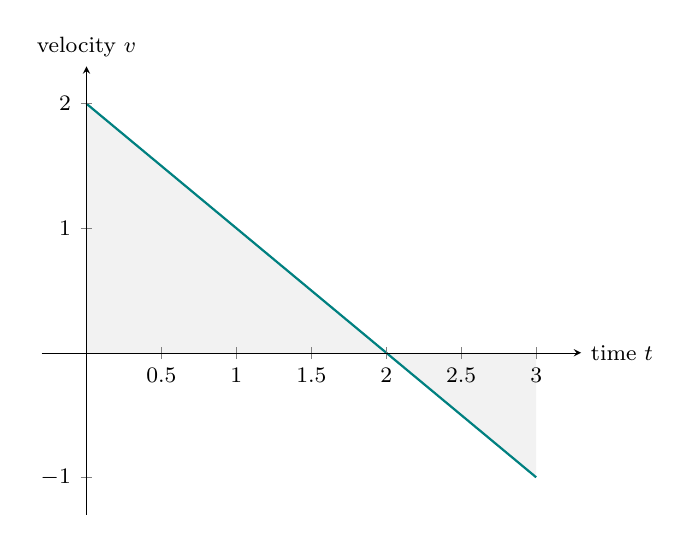
\begin{tikzpicture}
    \begin{axis}[
      axis on top,
      axis lines=middle,
      enlargelimits=true,
      xlabel={\footnotesize time \(t\)},
      xlabel style={at={(ticklabel* cs:1)}, anchor=west},
      ylabel={\footnotesize velocity \(v\)},
      ylabel style={at={(ticklabel* cs:1)}, anchor=south},
      axis line style = {very thin},
      % xticklabels={,,},
      % xtick={0,0.1,0.2,0.3,0.4,0.5,0.6},
      % ytick={-4,-3,-2,-1,0,1,2},
      % yticklabels={,,},
      % xticklabels={0,1,2,3,4,5,6},
      samples=500,
      smooth,
      no markers,
      ]
      \fill[gray!10] plot[domain=0:3] (\x,2-\x) -- (3,0) -- (0,0);
      \addplot[thick, smooth, teal, domain=0:3] {2 - x};
    \end{axis}
  \end{tikzpicture}
\end{document}
